\section{Experiments}
\label{sec:experiments}

All experiments are small numerical computations with our own scripts
(\cref{app:details} lists them). Unless stated otherwise, curves are
$f(x)=A\sqrt2\,\sin(w\pi x+\varphi)$ on $[-1,1]$ and data points are uniform on
$[-1,1]^2$, with $y$ independent of $x$. The default amplitude is $A=0.577$, the
standard deviation of the labels, so the peak is $p=A\sqrt2=0.816$. Each curve
is sampled as a polyline with consecutive samples at most $0.002$ apart along
the curve, and the distance from a point to the polyline is computed exactly.

\subsection{Frequency with everything else held fixed}
\label{sec:freq}

Earlier tests of the conjecture varied polynomial degree or network width, which
changes the output amplitude together with the squiggliness. Here the frequency
$w$ is the only variable: by \cref{cor:phase} the distribution of $f(x)$ at
every $x$ is identical in every row of \cref{tab:freq}. We use 3000 trials of
30 points each and 100 stratified random phases per frequency.

\begin{table}[t]
  \caption{Frequency isolation. Mean nearest-point distance and mean vertical
  error against frequency $w$, with the two lower bounds on the nearest-point
  distance: the mean vertical error divided by $\sqrt{1+K^2}$ with $K=p\,w\pi$
  (\cref{thm:sandwich}), and $4/(4l+4\sqrt\pi)$ (\cref{prop:length} with $V=4$).}
  \label{tab:freq}
  \centering
  \begin{tabular}{rrcccc}
    \toprule
    $w$ & arc length $l$ & nearest-point & vertical & bound, \cref{thm:sandwich} & bound, \cref{prop:length} \\
    \midrule
    0.25 &   2.19 & 0.6129 & 0.6672 & 0.5617 & 0.2524 \\
    0.5  &   2.66 & 0.4890 & 0.6664 & 0.4099 & 0.2256 \\
    1    &   3.96 & 0.3095 & 0.6649 & 0.2416 & 0.1744 \\
    2    &   6.96 & 0.1717 & 0.6651 & 0.1273 & 0.1145 \\
    4    &  13.32 & 0.0928 & 0.6663 & 0.0647 & 0.0663 \\
    8    &  26.26 & 0.0529 & 0.6678 & 0.0325 & 0.0357 \\
    16   &  52.31 & 0.0338 & 0.6665 & 0.0162 & 0.0185 \\
    32   & 104.50 & 0.0249 & 0.6657 & 0.0081 & 0.0094 \\
    64   & 208.92 & 0.0207 & 0.6688 & 0.0041 & 0.0047 \\
    \bottomrule
  \end{tabular}
\end{table}

\begin{figure}[t]
  \centering
  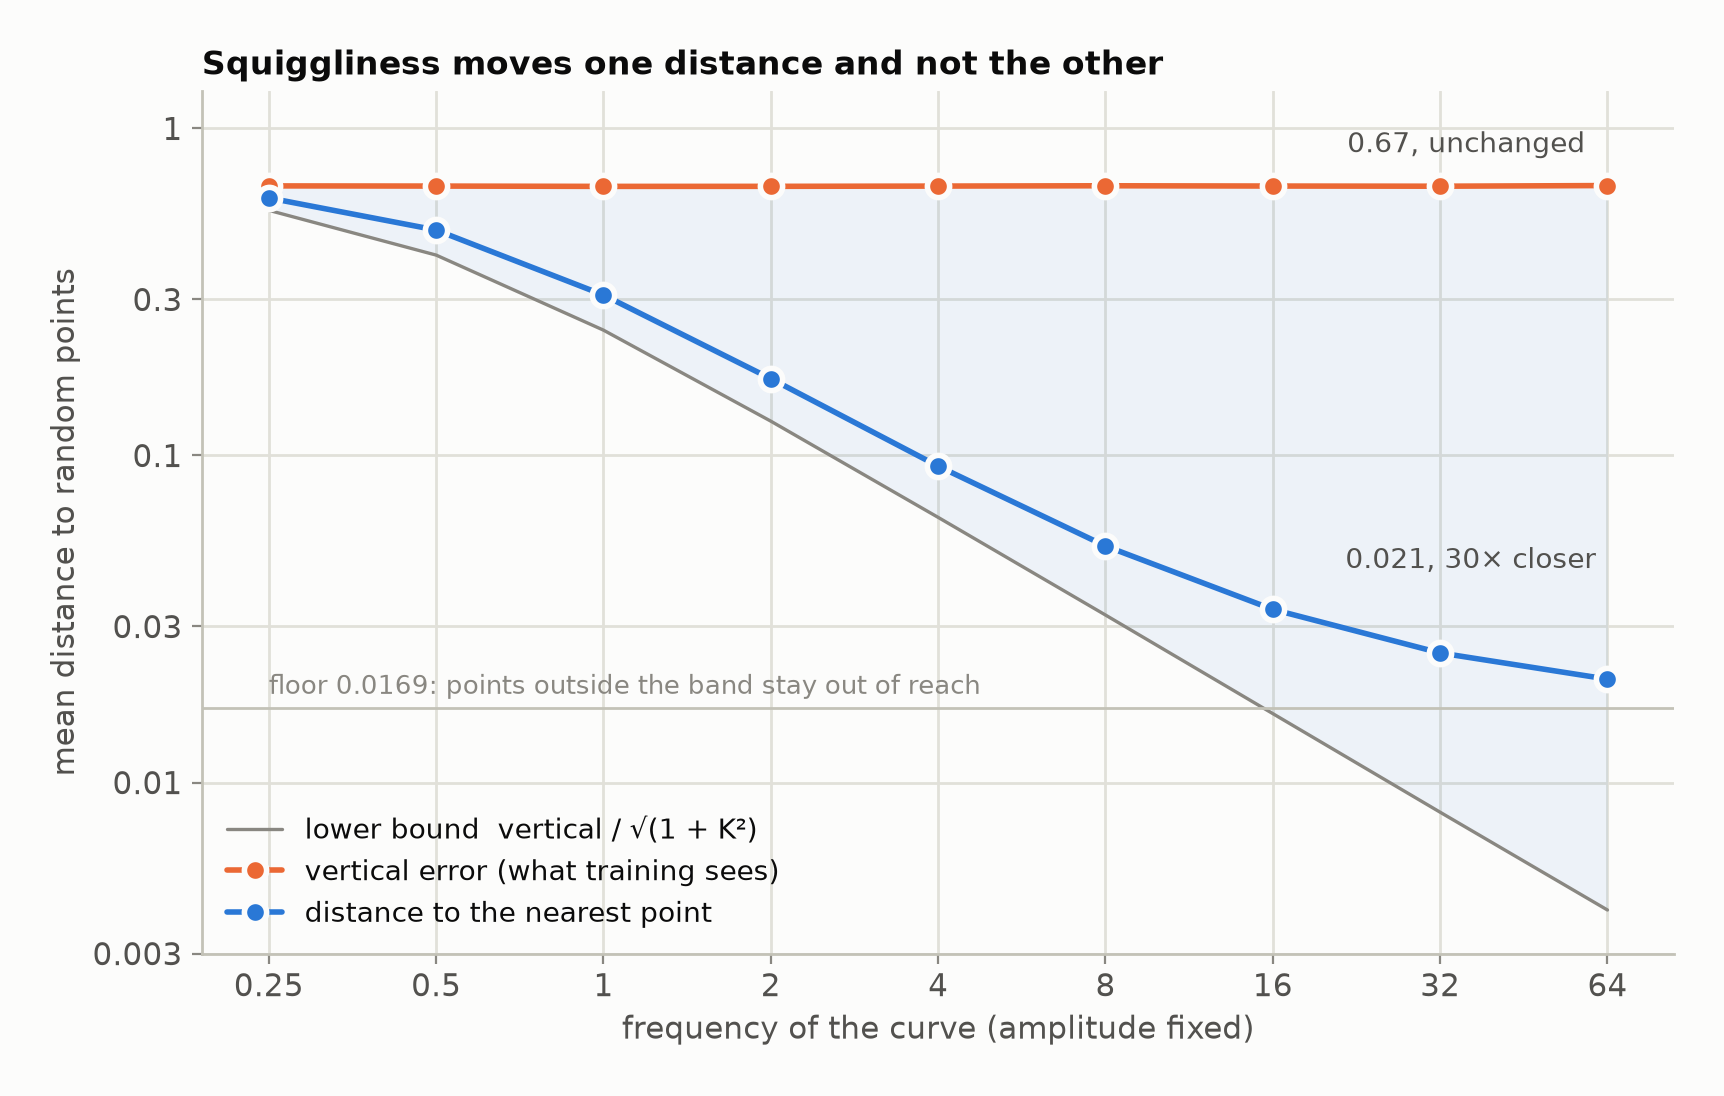
\includegraphics[width=0.72\linewidth]{../graphs/readme_frequency.png}
  \caption{The data of \cref{tab:freq}. The nearest-point distance (blue) falls
  with frequency and stays above the lower bound of \cref{thm:sandwich} (grey
  line). The vertical error (orange) does not move. The horizontal line is the
  floor $(1-p)^2/2=0.0169$ of \cref{prop:floor}.}
  \label{fig:freq}
\end{figure}

The nearest-point distance falls from $0.6129$ to $0.0207$, a factor of $29.6$.
Claim (G) holds, and not through amplitude. The vertical error lies between
$0.6649$ and $0.6688$ in every row, with no trend; the value predicted after
\cref{cor:phase} is $(1+p^2/2)/2=0.6665$. The flat column is \cref{cor:phase}
observed, and the differences between rows are sampling noise. Both lower bounds
hold in every row. At $w=64$ the function has Lipschitz constant $164$, and this
steepness is what \cref{thm:sandwich} requires for a nearest-point distance 32
times smaller than the vertical error. From $w=16$ the gap to both bounds
widens, because the distance approaches the floor of \cref{prop:floor}
(\cref{fig:freq}).

\subsection{A straight line of the same length}
\label{sec:line}

If length alone produced the effect, a straight segment of the same arc length
should score like the sine. We take $y=mx+b$ on $x\in[-1,1]$ with
$m=\sqrt{(l/2)^2-1}$, so that its length is $l$, and $b$ uniform on $[-1,1]$.

\begin{table}[t]
  \caption{Mean nearest-point distance for the sine and for a straight segment
  of the same length. The last two columns give the slope of the segment and
  the share of its length that lies outside the data box $[-1,1]^2$, averaged
  over $b$.}
  \label{tab:line}
  \centering
  \begin{tabular}{rrccrc}
    \toprule
    $w$ & arc length & sine & straight segment & slope $m$ & share outside the box \\
    \midrule
    4  &  13.32 & 0.0928 & 0.5022 &   6.6 & 85\% \\
    16 &  52.31 & 0.0338 & 0.5007 &  26.1 & 96\% \\
    64 & 208.92 & 0.0207 & 0.5006 & 104.5 & 99\% \\
    \bottomrule
  \end{tabular}
\end{table}

The segment stays at $0.50$ while the sine reaches $0.021$ (\cref{tab:line}).
This comparison needs a caveat. A segment of length $209$ over $x\in[-1,1]$ has
slope $104$, and about $99\%$ of it lies above or below the data. The part
inside the box has length about $2$ in all three rows, and a near-vertical
segment of length $2$ through the middle of the box has mean distance
$\E|x|=0.5$. The table therefore shows that length outside the data region is
worth nothing. It does not show that length is irrelevant: by
\cref{prop:length}, length is necessary, and the sine achieves its small
distance because its length is inside the box and spread across it.

\subsection{What sets the floor}
\label{sec:saturation}

An earlier version of this work predicted that the distance stops falling once
the wavelength $2/w$ drops below the mean spacing $2/n$ of $n$ data points, so
that the knee of the curve $D(w)$ would sit at $w^\ast\propto n$. We swept
$n\in\{10,30,100,300,1000\}$ and 25 frequencies in $[1,1000]$ with $30\,000$
points per $n$, and located the knee by two criteria fixed in advance: the
breakpoint of a continuous two-segment fit of $\log D$ on $\log w$, and the
smallest $w$ at which doubling $w$ lowers $D$ by less than $10\%$.

\begin{table}[t]
  \caption{Knee frequency $w^\ast$ against the number of points $n$. The
  prediction under test was slope $1$ of $\log w^\ast$ on $\log n$. Confidence
  intervals are from a bootstrap over trials.}
  \label{tab:knee}
  \centering
  \begin{tabular}{lcccccrc}
    \toprule
    criterion & $n=10$ & 30 & 100 & 300 & 1000 & slope & 95\% interval \\
    \midrule
    two-segment fit      & 21.6 & 21.6 & 21.6 & 21.6 & 21.6 & $-0.000$ & $[-0.004,\,0.004]$ \\
    doubling gains $<10\%$ & 60.1 & 61.7 & 61.4 & 61.0 & 59.4 & $-0.003$ & $[-0.014,\,0.008]$ \\
    \bottomrule
  \end{tabular}
\end{table}

The slope is $0$, not $1$ (\cref{tab:knee}), and the five curves $D(w)$ agree to
within $3.1\%$ at every frequency. No experiment was needed for this: the
quantity is a mean of per-point distances, so its expectation cannot depend on
$n$. What sets the knee is the band edge of \cref{prop:floor}. With $p=0.816$
the floor is $D_\infty=(1-p)^2/2=0.0169$, and a fit of
$D-D_\infty=c\,w^{-\beta}$ for $w\ge20$ gives $\beta=0.990$ and $c=0.248$. For
$D=D_\infty+c/w$ the $10\%$ criterion triggers at $c(1-2r)/(2rD_\infty)=58.6$
with $r=0.1$, against $59$ to $62$ measured.

As a control we set $A\sqrt2=1$, so that the band covers the data and the floor
is zero. The saturation disappears (\cref{fig:floor}): the distance follows
$0.301\,w^{-1.002}$ up to $w=1000$, where it is $0.00030$, and the $10\%$
criterion never triggers.\footnote{The two-segment fit still reports a
breakpoint, at $1.8$, because it always returns one.} \Cref{prop:sine} predicts
$w\,D_1(w)\to0.2974$. The repository reports $0.2965$ at $w=256$; a separate run
for this paper, with $40\,000$ points and 8 phases, gave $0.298$ at $w=64$ and
at $w=256$, and $D\,l=1.192$ against the predicted $1.189$.

\begin{figure}[t]
  \centering
  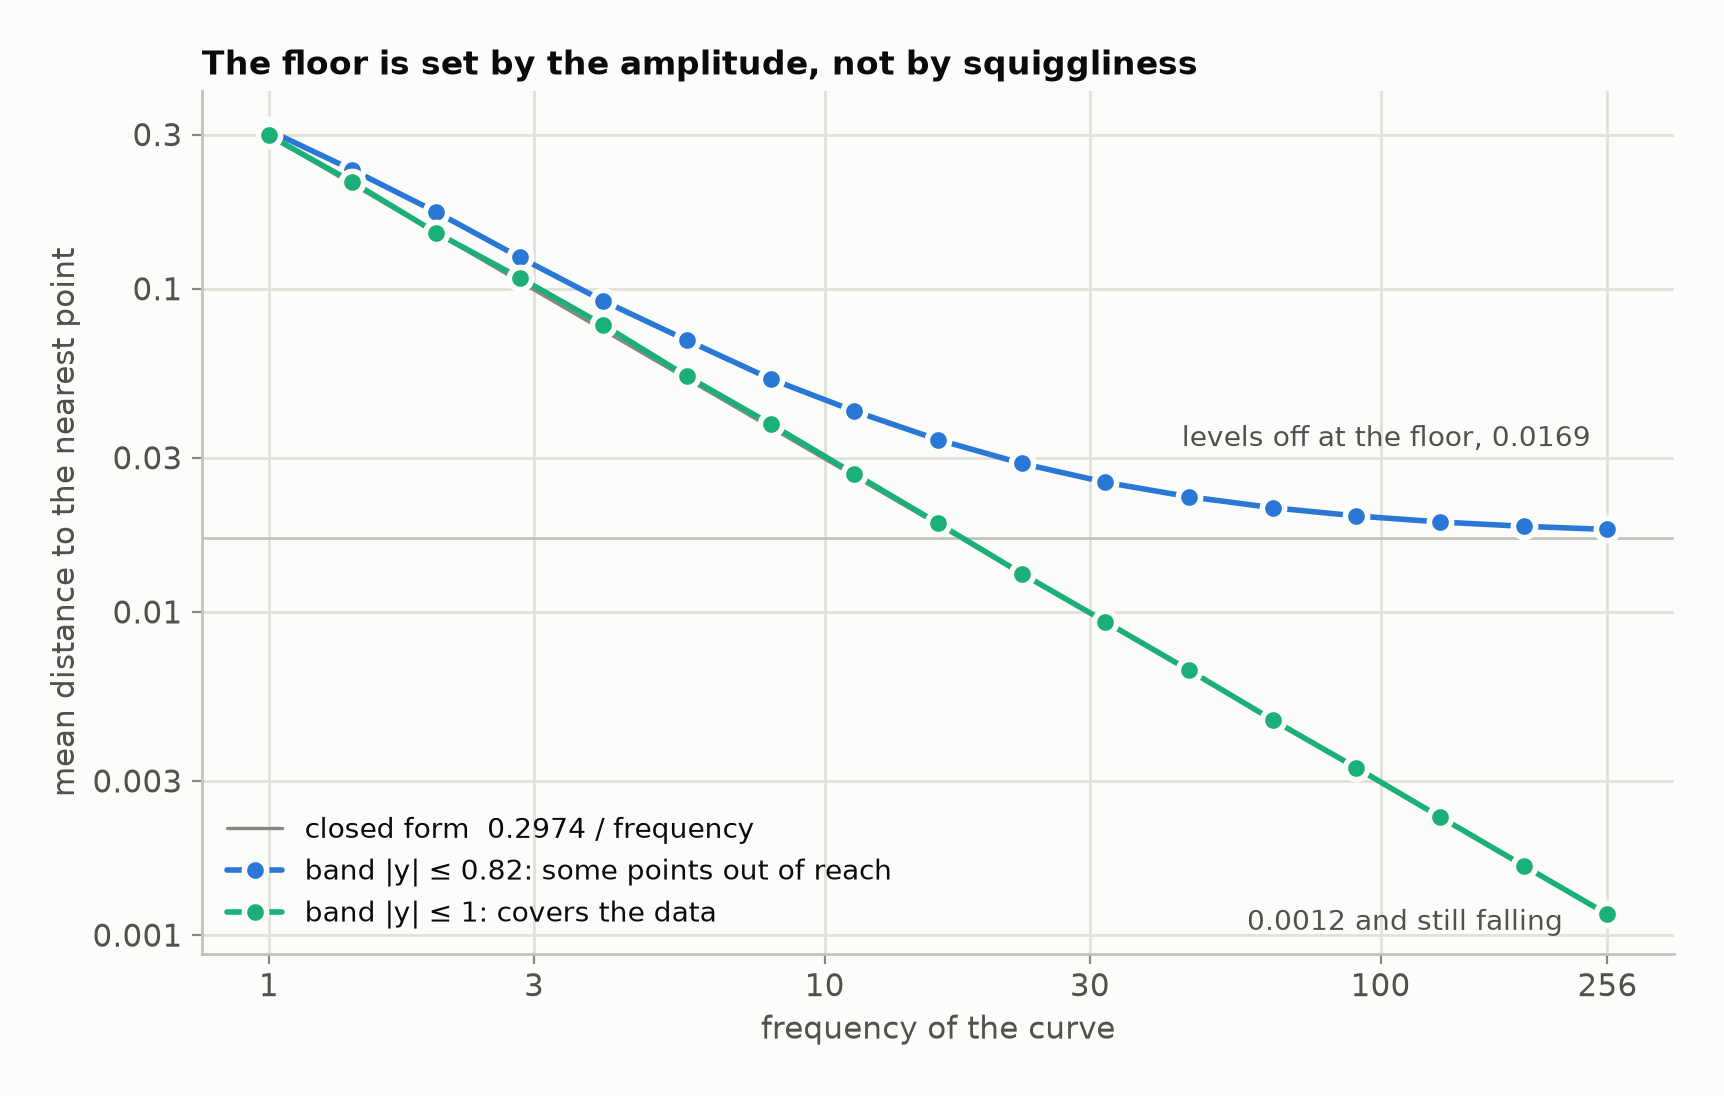
\includegraphics[width=0.72\linewidth]{../graphs/readme_floor.png}
  \caption{The floor comes from the amplitude. Blue: default amplitude, band
  $|y|\le0.82$; the distance levels off at $0.0169$. Green: band $|y|\le1$; no
  floor, and the distance follows the constant of \cref{prop:sine} (grey line,
  under the green one).}
  \label{fig:floor}
\end{figure}

\subsection{Random networks}
\label{sec:nets}

\paragraph{Initial loss against width.} We draw 200 points with $x$ uniform on
$[-1,1]^{10}$ and $y$ uniform on $[-1,1]$, and for each width 200 untrained
ReLU networks with two hidden layers and no biases, as in \cref{cor:he}. The
prediction of \cref{cor:he}, evaluated on the sample, is the mean of
$y^2+2\|x\|^2/d$, which is $1.03$.

\begin{table}[t]
  \caption{Mean squared error before training, 200 networks per width
  ($\pm$ one standard error). Predictions are from \cref{cor:he}.}
  \label{tab:mse}
  \centering
  \begin{tabular}{rcccc}
    \toprule
    & \multicolumn{2}{c}{He initialisation} & \multicolumn{2}{c}{$N(0,1)$ weights} \\
    \cmidrule(lr){2-3}\cmidrule(lr){4-5}
    width & measured & predicted & measured & predicted \\
    \midrule
       4 & $1.07\pm0.12$ & 1.03 & $15$ & $14$ \\
      16 & $1.02\pm0.05$ & 1.03 & $220$ & $219$ \\
      64 & $1.07\pm0.04$ & 1.03 & $3.45\times10^{3}$ & $3.51\times10^{3}$ \\
     256 & $1.10\pm0.04$ & 1.03 & $6.02\times10^{4}$ & $5.61\times10^{4}$ \\
    1024 & $1.03\pm0.04$ & 1.03 & $8.23\times10^{5}$ & $8.97\times10^{5}$ \\
    \bottomrule
  \end{tabular}
\end{table}

A wider network does not start closer (\cref{tab:mse}; \cref{fig:mse} in \cref{app:details}). The measured
values scatter around the prediction; the largest deviation, at width 256, is
$1.9$ standard errors. With unscaled weights a wider network starts much further
away, because its output grows with width. That growth is an amplitude effect,
and it is the confound that the design of \cref{sec:freq} removes.

\paragraph{Curve length against width and depth.} For claim (P) we look at the
curves themselves, for a one-dimensional input. Each network has He-uniform
weights and hidden biases uniform on $[-0.5,0.5]$, and its output is shifted and
scaled so that its range over $[-1,1]$ is exactly $[-1,1]$. We measure arc
length, the number of turns (sign changes of the slope), and the mean
nearest-point distance to 200 fixed random points, over 300 networks per size.

Width adds turns and no length (\cref{tab:relu-full} in \cref{app:details}).
From width 2 to 512, with two hidden layers, the mean number of turns rises
from $0.5$ to $15$, the arc length stays between $3.4$ and $3.6$, and the
nearest-point distance is flat from width 16, between $0.42$ and $0.43$. Depth
adds some length: from 1 to 16 layers at width 64 the arc length rises from
$3.4$ to $5.1$ and the distance falls from $0.44$ to $0.34$. For comparison,
the same code gives length $4.61$ and distance $0.351$ for a sine with one
period across the box, and $64.07$ and $0.021$ for a sine with 16 periods. Even
at depth 16 the random curves resemble the first and not the second. So claim
(P) fails for width and holds weakly for depth.

This measurement has caveats. The input is one-dimensional. Rescaling the output
controls the amplitude but does not hold the marginals of $f(x)$ fixed, unlike
\cref{sec:freq}. Only the nearest-point distance is measured, not the vertical
error. The distances use a fixed grid of 4001 samples, which overestimates the
distance by about $7\%$ for the sine with 16 periods ($0.0209$ against $0.0196$
with exact projection). Finally, the rescaling and the biases mean that the
depth trend is not directly comparable with the theorem of
\citet{hanin2022preserve} discussed in \cref{sec:related}.
